\section{Data Description}
\label{sec:data-description}
\subsection{Data Sources}
The datasets needed for the exploration of the time series and the fitting of the models have been obtained from the ESIOS -- System Operator's Electronic Information System. This is an online portal where the System Operator, the REE -- Spanish Electrical Grid -- uploads all relevant information for the operation of the grid. 

In order to accomplish everything outlined in \autoref{sec:objective-and-scope} six different datasets are needed. These datasets are:
\begin{itemize}
    \item Real time wind energy hourly generation
    \item Real time solar PV energy hourly generation
    \item Real time solar thermal energy hourly generation
    \item Wind energy monthly installed capacity
    \item Solar PV energy monthly installed capacity
    \item Solar thermal energy monthly installed capacity
\end{itemize}

%\href{https://www.esios.ree.es/es/analisis/551?vis=1&start_date=26-08-2024T00%3A00&end_date=26-08-2024T23%3A55&compare_start_date=25-08-2024T00%3A00&groupby=minutes5}{https://www.esios.ree.es/es/analisis/551}
%\href{https://www.esios.ree.es/es/analisis/1295?vis=1&start_date=26-08-2024T00%3A00&end_date=26-08-2024T23%3A55&compare_start_date=25-08-2024T00%3A00&groupby=minutes5}{https://www.esios.ree.es/es/analisis/1295}
%\href{https://www.esios.ree.es/es/analisis/1294?vis=1&start_date=26-08-2024T00%3A00&end_date=26-08-2024T23%3A55&compare_start_date=25-08-2024T00%3A00&groupby=minutes5}{https://www.esios.ree.es/es/analisis/1294}

\subsection{Data Preprocessing}
The obtained datasets are already very clean, so no missing or obviously wrong values were found on any of them. The installed capacity is obtained on a monthly basis as there is not any lower granularity in the ESIOS portal. With this datasets, the capacity factor is obtained as explained in equation \eqref{eq:capacity-factor} by dividing the generated electricity by the installed capacity times the period time frame. The time frame in this case is always one hour. Like this the hourly capacity factor for the Spanish electrical system for the three different technologies is obtained. Note that the data obtained spans from mid 2015 until end of 2023, since no previous data is available. 

\subsection{Exploratory data analysis}

Now that it is well understood where the data comes from, an initial analysis of the data to understand what the capacity factor of each looks like will be performed. 

\subsubsection{Initial visualization}
The first variable to be visualized will be that of the solar PV capacity factor, which can be seen in 
\begin{figure}[ht]
    \centering
    \captionsetup{justification=centering}
    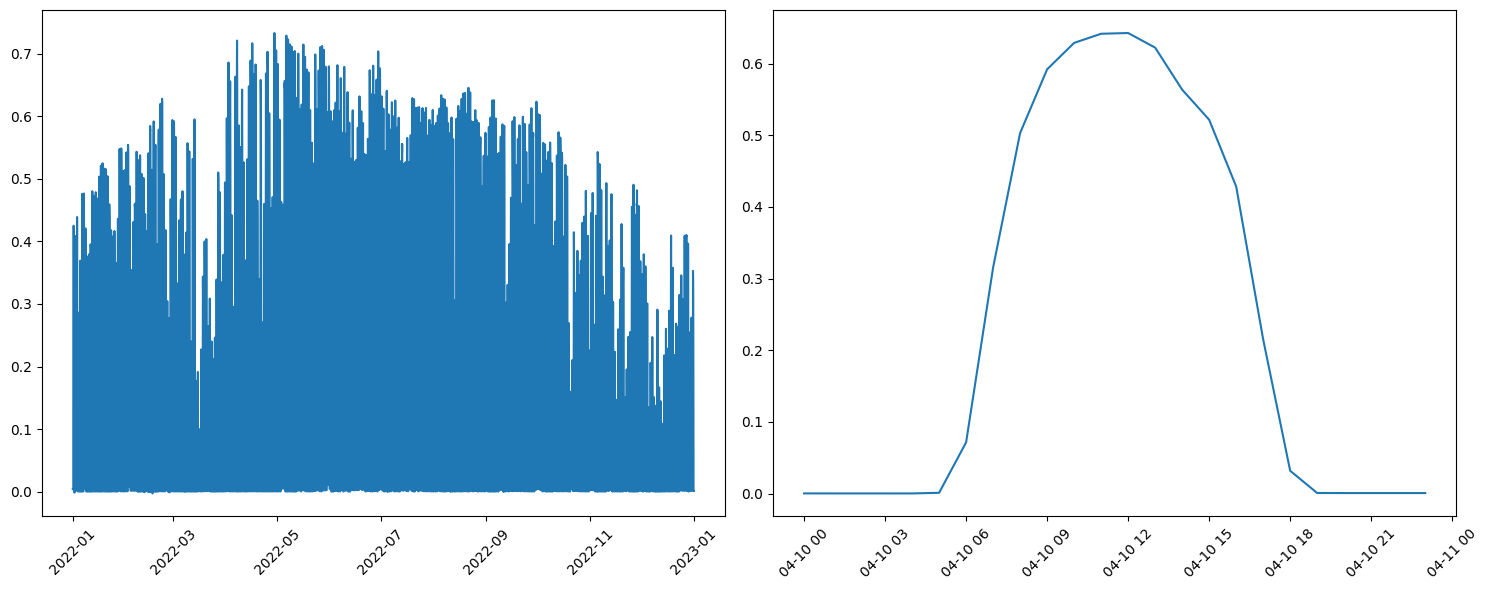
\includegraphics[width=\linewidth]{assets/spv-year-day.png}
    \caption{Yearly and daily profiles of the solar PV capacity factor, taken for 2022 and the 10\textsuperscript{th} April 2022 respectively.}
    \label{fig:spv-year-day}
\end{figure}

The main features of the series can be well visualized here. The yearly seasonality is very clear, with higher peak values in summer and lower peak values in winter, although this is altered by periods of lower sunlight where peaks are reduced below the typical seasonal peak, like at the beginning of March. The daily pattern is also very clear, with values of practically zero -- it is not exactly zero due to some background light and noise in the measurement -- at night and a generation in accordance with the position of the sun in its ecliptic. 

The solar thermal profile, although belonging to the same renewable resource as the solar PV, is slightly different. 
\begin{figure}[ht]
    \centering
    \captionsetup{justification=centering}
    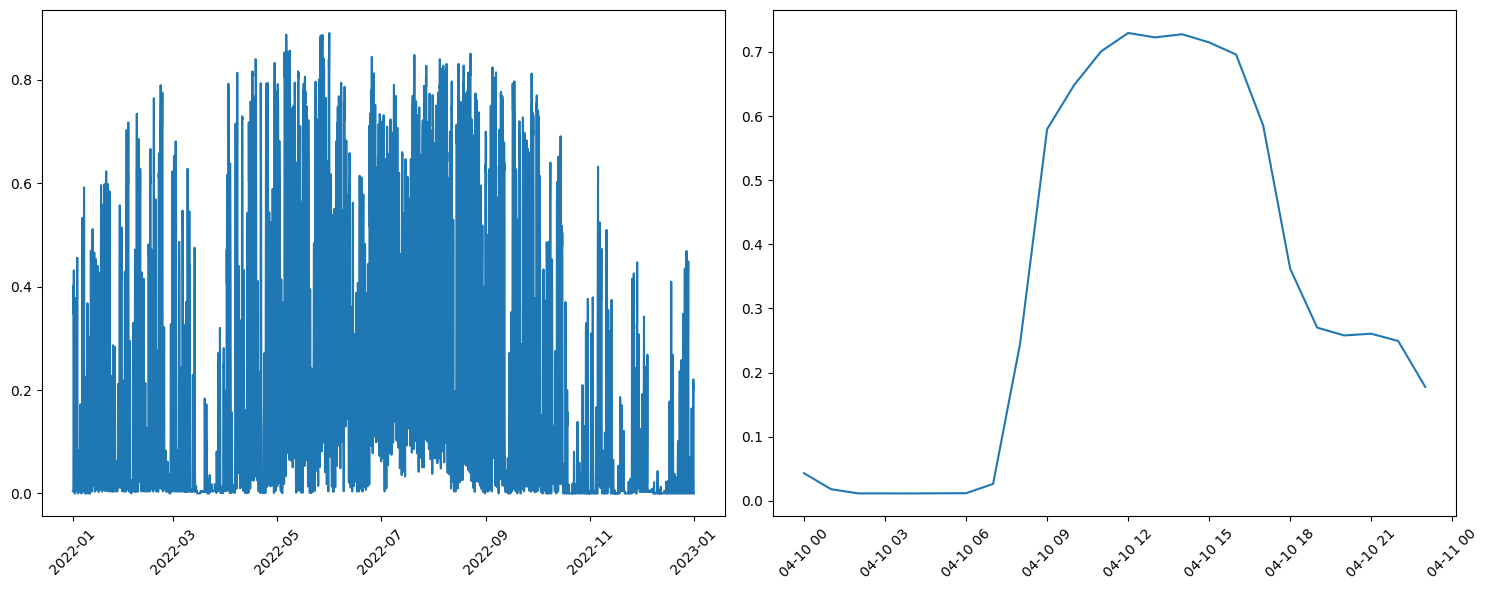
\includegraphics[width=\linewidth]{assets/st-year-day.png}
    \caption{Yearly and daily profiles of the solar thermal capacity factor, taken for 2022 and the 10\textsuperscript{th} April 2022 respectively.}
    \label{fig:st-year-day}
\end{figure}

Several differences between these profiles shown in \autoref{fig:st-year-day} and the previous ones are apparent. The yearly pattern, even though it follows roughly the same seasonality with higher peaks in summer is much more volatile than that of the solar PV. Furthermore, there are whole periods of several days where generation does not go to zero, due to the inertia of the thermal system. The highest peaks are also whigher for the solar thermal, reaching generation values much closer to its rated capacity in the summer than the solar PV. In the daily pattern the mentioned inertia can be clearly seen, where appart from the general sinusoidal throughout the day it can be seen how generation remains above zero at night.

\begin{figure}[ht]
    \centering
    \captionsetup{justification=centering}
    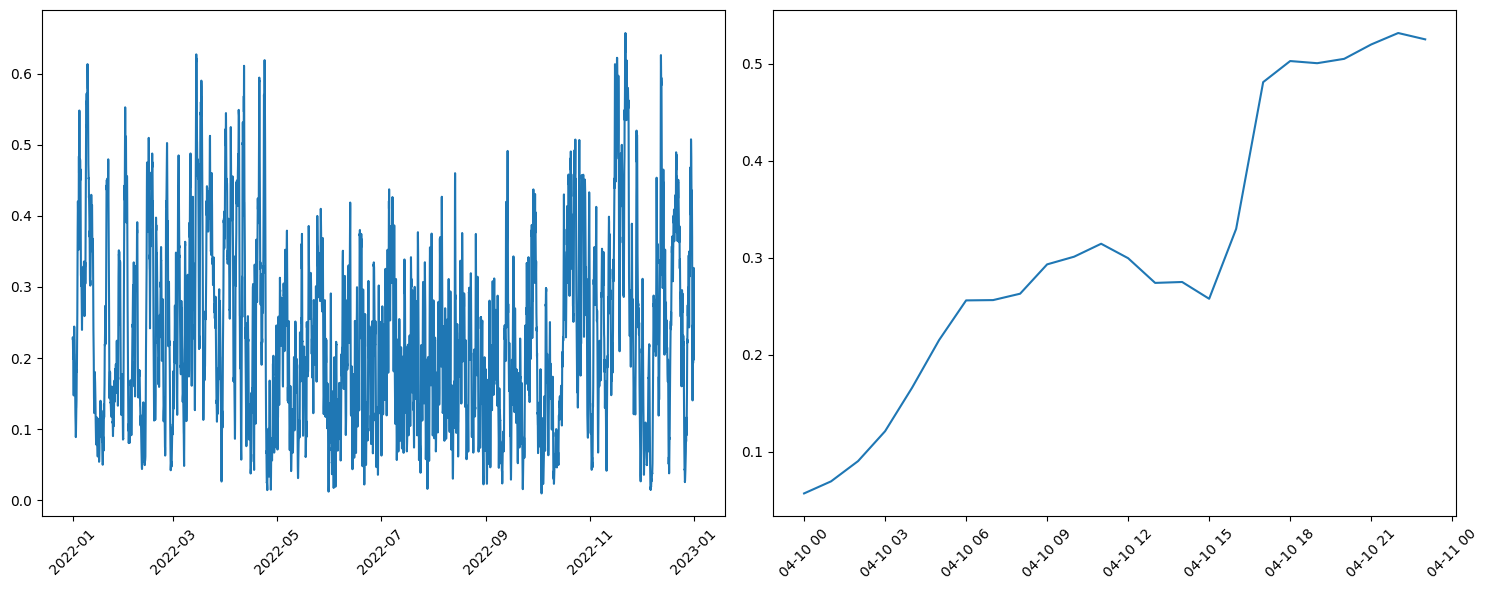
\includegraphics[width=\linewidth]{assets/w-year-day.png}
    \caption{Yearly and daily profiles of the wind capacity factor, taken for 2022 and the 10\textsuperscript{th} April 2022 respectively.}
    \label{fig:w-year-day}
\end{figure}

The wind profile shown in \autoref{fig:w-year-day} is the most different of the three. The yearly profile is the most volatile of the three, with less of a clear seasonal pattern although it can be seen how the mean values in summer seem to be lower than those in the winter. In the daily profile there are not any obvious patterns which can be seen at first view. 

